\documentclass[12pt]{report}
\usepackage{graphicx}
\usepackage{hyperref}
\usepackage{geometry}
\usepackage{amsmath}
\usepackage{booktabs}
\usepackage{longtable}
\usepackage{array}
\usepackage{float}
\usepackage{caption}
\usepackage{listings}
\usepackage{setspace}
\geometry{margin=1in}
\onehalfspacing

\graphicspath{{../deliverables_outputs/visuals/}{../deliverables_outputs/powerbi_exports/screenshots/}}

\lstset{
  language=Python,
  basicstyle=\small\ttfamily,
  keywordstyle=\bfseries,
  commentstyle=\itshape,
  stringstyle=\ttfamily,
  showstringspaces=false,
  breaklines=true,
  frame=single
}

\title{Nodes and Nations: A Complex Network Study of Global Migration}
\author{Student Name (ID) \\ Department, University}
\date{April 2026}

\begin{document}
\maketitle

\begin{abstract}
This study models global migration as a dynamic directed weighted network using UN DESA bilateral stocks and socio-economic indicators. The core contribution is a temporal corridor analysis that converts origin--destination stocks into interval-based dynamics (1995--2000 to 2020--2024), revealing persistent versus shock-driven routes. Centrality metrics identify destination hubs and bridge nodes; community detection exposes regional migration systems; regression links flows to economic scale, conflict, climate pressure, and policy openness. A Migration Influence Score (MIS), combining PageRank with total flow, highlights structurally influential high-volume hubs. The result is an interpretable, policy-relevant account of how migration systems are organized and how they evolve.
\end{abstract}

\section*{Executive Summary}
\begin{itemize}
  \item \textbf{Structural concentration:} a small destination core dominates global inflows, revealing a hub-dominated system rather than dispersed connectivity.
  \item \textbf{Temporal persistence with shocks:} major corridors persist across intervals, while conflict-driven routes surge and become embedded in regional systems.
  \item \textbf{Regional systems:} community structure aligns with geography and labor markets, indicating stable blocs with limited cross-bloc bridging.
  \item \textbf{Drivers with policy leverage:} economic scale pulls migrants into hubs, while conflict and climate push outflows; visa openness amplifies corridor intensity.
\end{itemize}

\tableofcontents
\listoffigures
\listoftables
\newpage

\chapter{Introduction}
International migration shapes labor markets, demography, and development at a scale that cannot be explained by bilateral tables alone. Traditional origin--destination summaries describe volume but miss system-level interactions, feedback effects, and corridor dependencies. A network perspective captures these interactions and reveals how hubs, bridges, and regional blocs structure global mobility. This report builds a temporal migration network to extract structural patterns and interpret their real-world meaning.

\section*{What problem is addressed on this page}
\begin{itemize}
  \item \textbf{Problem:} bilateral tables hide global structure. \textbf{Solved by:} modeling migration as a network to surface hubs, bridges, and blocs.
  \item \textbf{Problem:} trends are reported without mechanism. \textbf{Solved by:} linking temporal snapshots to structural measures.
\end{itemize}

\chapter{Literature Motivation: Why Network Science for Migration}
Migration systems are relational: corridor choices affect other corridors through substitution, chain migration, and policy spillovers. A network perspective improves interpretability, allows comparison over time, and links structural measures to policy outcomes such as corridor resilience and shock propagation.

\section*{What problem is addressed on this page}
\begin{itemize}
  \item \textbf{Problem:} corridor-by-corridor analysis cannot explain system-wide shifts. \textbf{Solved by:} network measures that capture interdependence.
  \item \textbf{Problem:} policy impact is hard to localize. \textbf{Solved by:} mapping influence and clustering to identify leverage points.
\end{itemize}

\chapter{Objectives}
\begin{itemize}
  \item Construct temporal directed weighted migration networks from UN DESA bilateral stocks.
  \item Analyze interval-based migration corridors and identify persistent vs. emerging routes.
  \item Compute centrality metrics to identify hubs and bridge countries.
  \item Detect communities using Louvain, Girvan--Newman, and Leiden methods.
  \item Model migration drivers using regression with socio-economic and policy factors.
  \item Produce dashboard-ready outputs for policy visualization and reporting.
\end{itemize}

\chapter{Dataset Description}
\section{UN DESA Migration Data}
The primary dataset is the UN DESA International Migrant Stock (IMS), which provides bilateral origin--destination stocks by year. Data are converted from matrix form into long-format records with origin, destination, year, and migrant stock.

\section{Supplementary Datasets}
Auxiliary indicators align with origin and destination countries and include GDP, population, unemployment, education proxies, conflict intensity, climate risk, and visa openness. These variables enable explanatory modeling of migration flows and interpretive context for network results.

\chapter{Data Preprocessing}
Data preprocessing standardizes country identifiers, removes aggregates, and enforces numeric consistency across years. Missing values are imputed with median values when used in regression.

\begin{lstlisting}
import pandas as pd

# Load and reshape UN DESA matrix to long format
df = pd.read_excel("undesa_pd_2024_ims_stock_by_sex_destination_and_origin.xlsx")
long_df = df.melt(id_vars=["destination"], var_name="origin", value_name="migrants")

# Clean and filter
long_df = long_df[long_df["migrants"].fillna(0) > 0]
long_df["migrants"] = long_df["migrants"].astype(float)
\end{lstlisting}

\chapter{Network Construction}
Each snapshot is a directed weighted graph $G=(V,E)$ where nodes are countries and edge weights are migration stocks. Self-loops are removed, edges are aggregated by origin--destination pairs, and weights preserve corridor intensity to avoid flattening high-volume routes. This design retains asymmetry (origin vs. destination roles) and supports both centrality and community detection on comparable snapshots.

\begin{lstlisting}
import networkx as nx

G = nx.DiGraph()
edges = long_df.groupby(["origin", "destination"], as_index=False)["migrants"].sum()
for _, row in edges.iterrows():
    if row["origin"] != row["destination"]:
        G.add_edge(row["origin"], row["destination"], weight=row["migrants"])
\end{lstlisting}

\chapter{Temporal Migration Analysis}
\section{Interval-Based Corridor Analysis}
The temporal analysis segments migration flows into six intervals: 1995--2000, 2000--2005, 2005--2010, 2010--2015, 2015--2020, and 2020--2024. For each interval, the top corridors are ranked by total stock and visualized. This isolates structural persistence from transient spikes, allowing corridor dynamics to be interpreted in relation to labor demand, policy shifts, and geopolitical shocks.

\section{Persistent vs. Emerging Corridors}
Persistent corridors (e.g., Mexico $\rightarrow$ USA, India $\rightarrow$ UAE) remain dominant across multiple intervals, reflecting long-run labor-market complementarities, diaspora network effects, and institutionalized mobility channels. Emerging corridors surface in later intervals, often associated with conflict displacement, regional crises, and policy shifts. This temporal lens emphasizes path dependence while capturing new geopolitical realities.

\section{Case Study: Syria to T\"urkiye}
The Syria $\rightarrow$ T\"urkiye corridor exemplifies a shock-driven surge that becomes structurally embedded. Conflict displacement increases volume quickly, and geographic proximity, policy responses, and logistical accessibility sustain the corridor over multiple intervals. In network terms, the edge weight rises sharply and remains salient among top corridors, illustrating how exogenous shocks can reconfigure regional migration systems.

\section{Real-World Implications}
Persistent corridors imply structural dependence between origin and destination economies, reinforcing policy continuity and bilateral planning. Emerging corridors indicate shifting pressures, requiring adaptive migration policy, labor agreements, and humanitarian planning. The interval-based approach demonstrates that changes are not random fluctuations but reflect identifiable political and economic drivers.

\section*{Insight Summary}
\begin{itemize}
  \item \textbf{Observation:} top corridors recur across intervals. \textbf{Pattern:} persistence dominates turnover. \textbf{Meaning:} long-run labor demand and diaspora networks anchor global mobility.
  \item \textbf{Observation:} shock-driven corridors surge in specific intervals. \textbf{Pattern:} rapid edge-weight growth. \textbf{Meaning:} displacement shocks reconfigure regional systems and remain visible over time.
  \item \textbf{Observation:} interval totals rise unevenly. \textbf{Pattern:} stepwise increases. \textbf{Meaning:} growth is driven by discrete geopolitical and policy shifts, not smooth trends.
\end{itemize}

\begin{figure}[H]
  \centering
  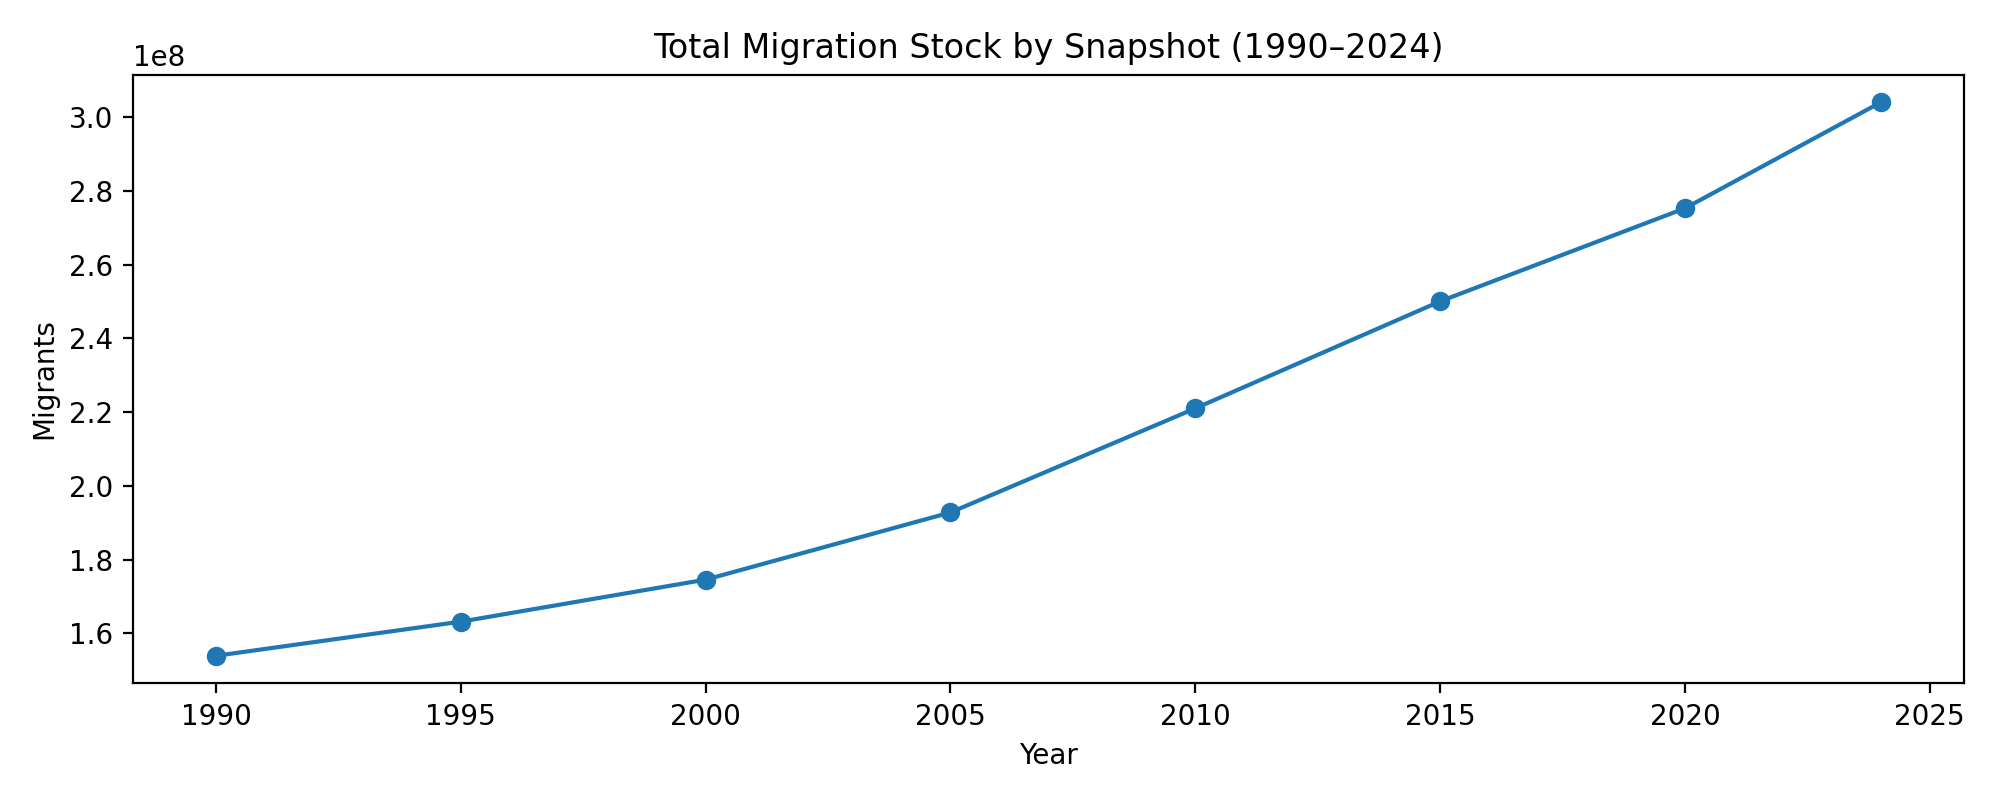
\includegraphics[width=0.95\textwidth]{interval_total_trend.png}
  \caption{Global migration totals by interval.}
\end{figure}

\begin{figure}[H]
  \centering
  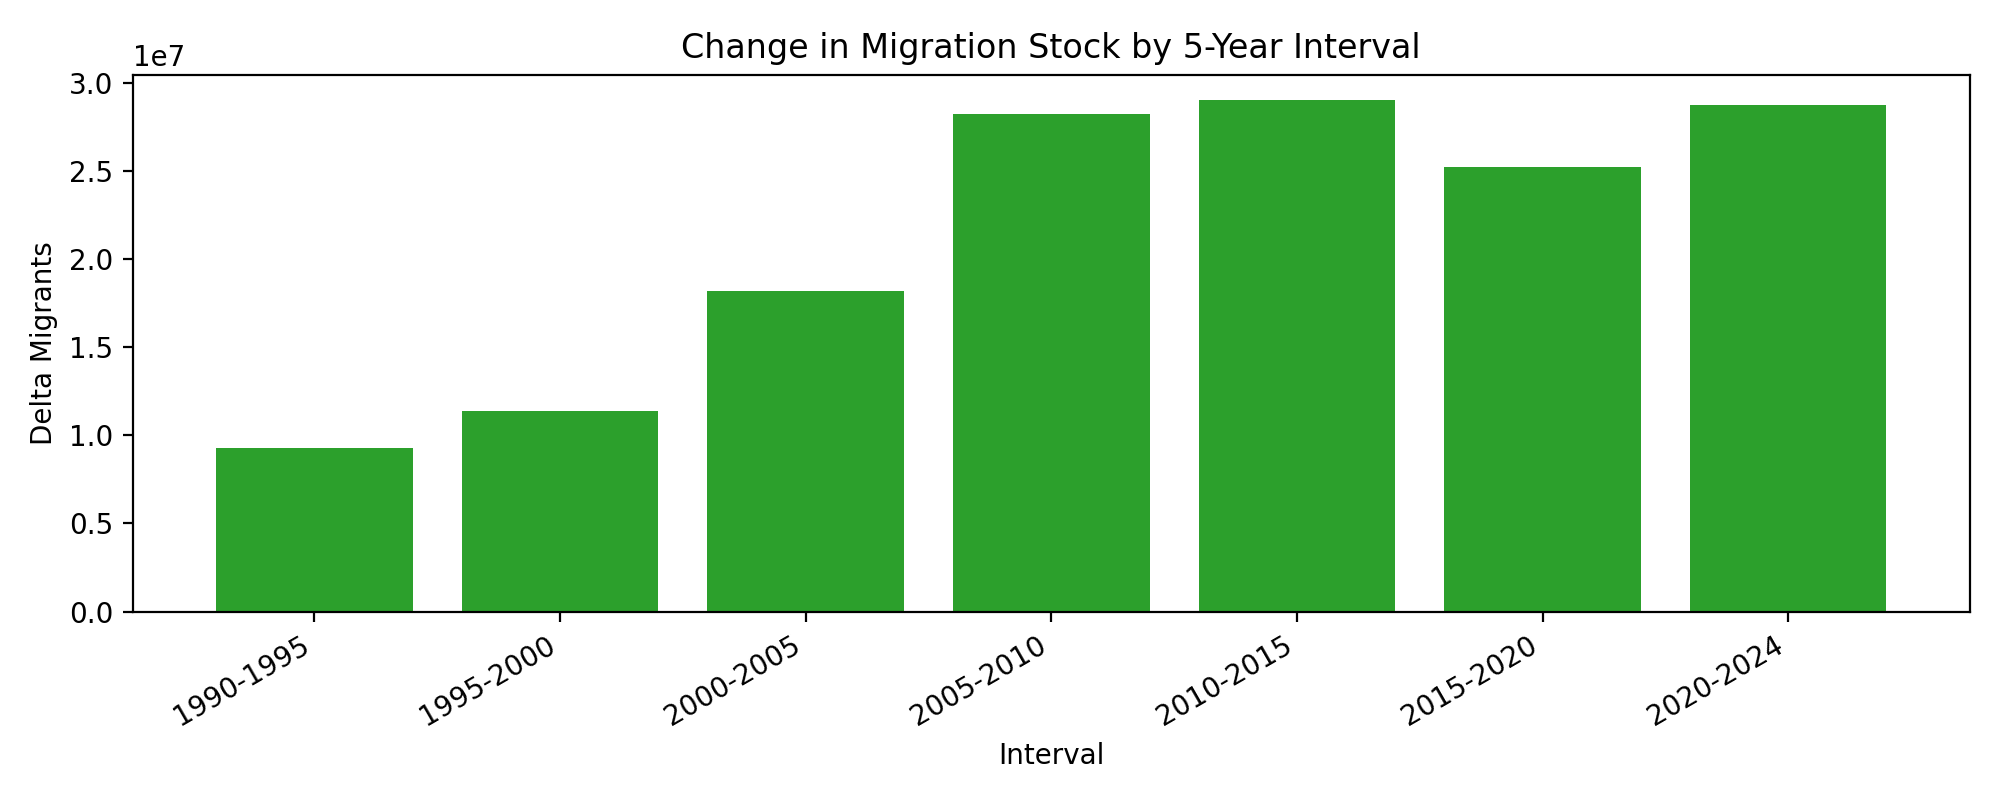
\includegraphics[width=0.95\textwidth]{interval_delta_bar.png}
  \caption{Interval-to-interval changes in total migration.}
\end{figure}

\begin{figure}[H]
  \centering
  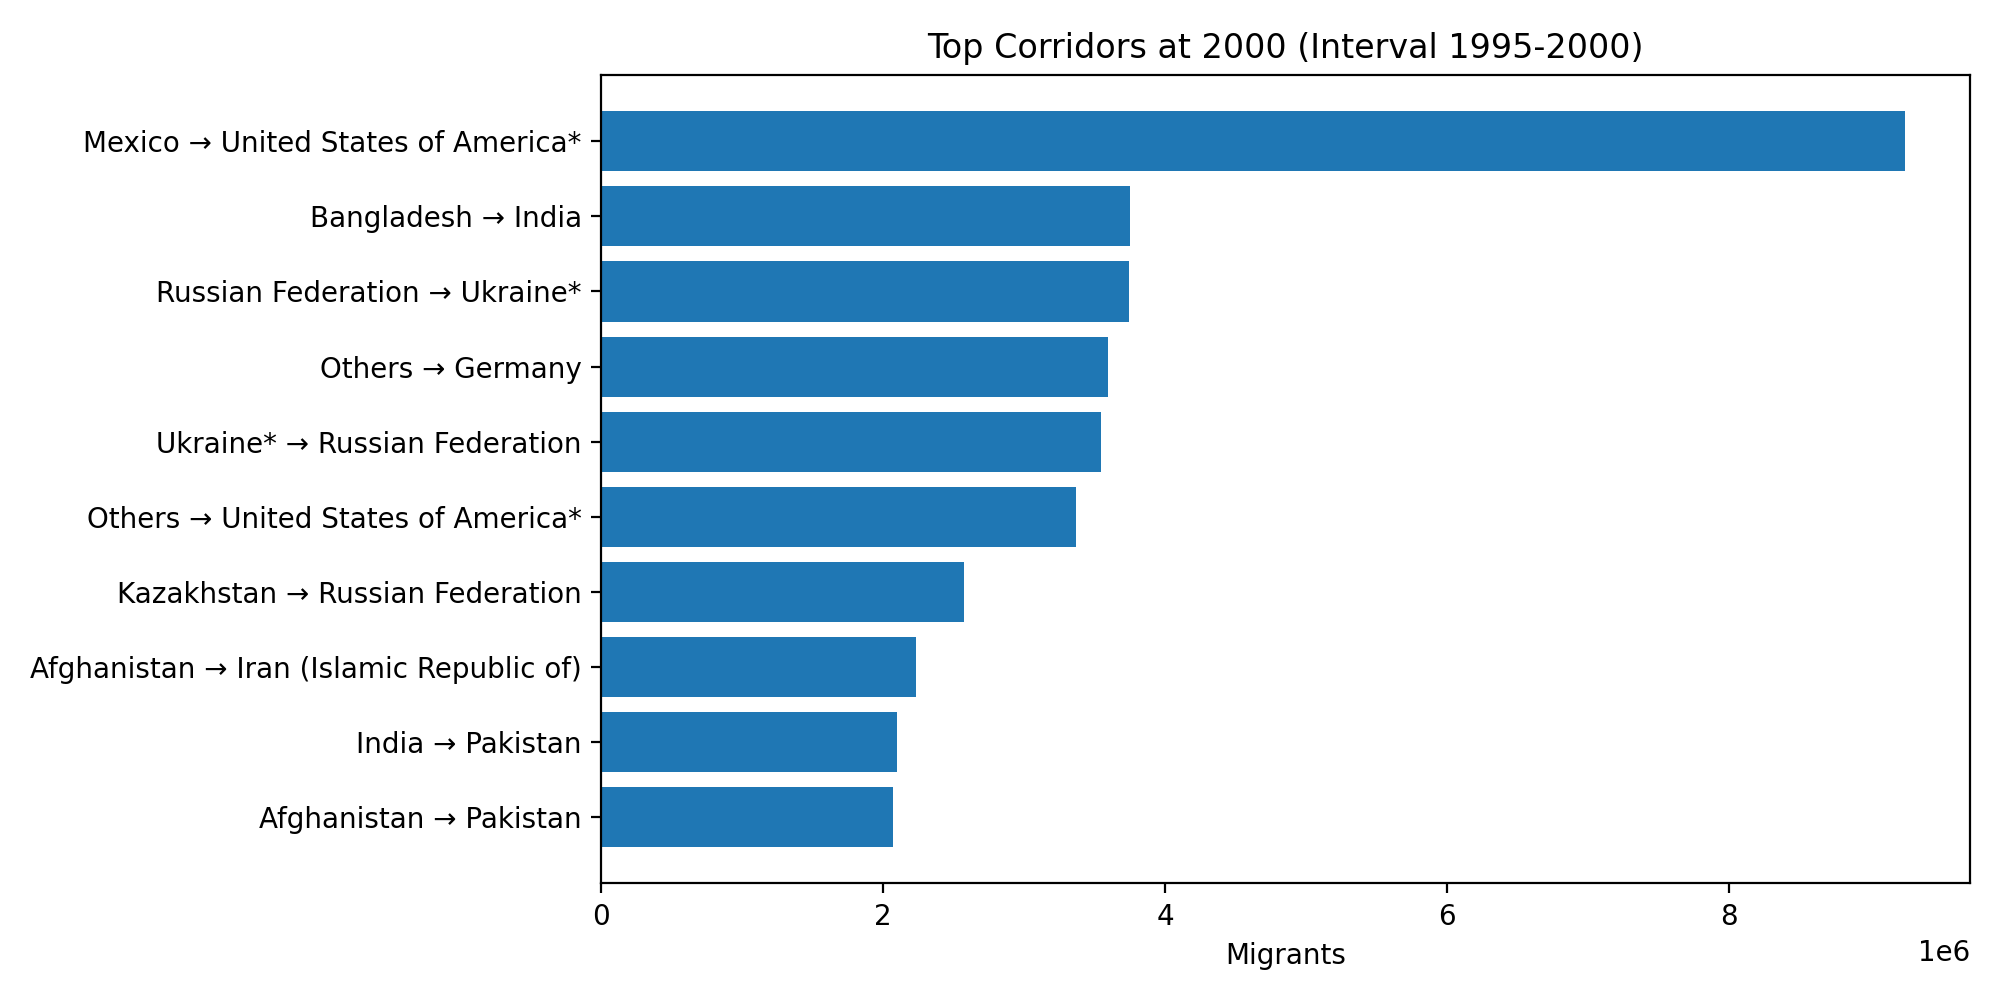
\includegraphics[width=0.95\textwidth]{interval_top_corridors_1995_2000.png}
  \caption{Top migration corridors, 1995--2000.}
\end{figure}

\begin{figure}[H]
  \centering
  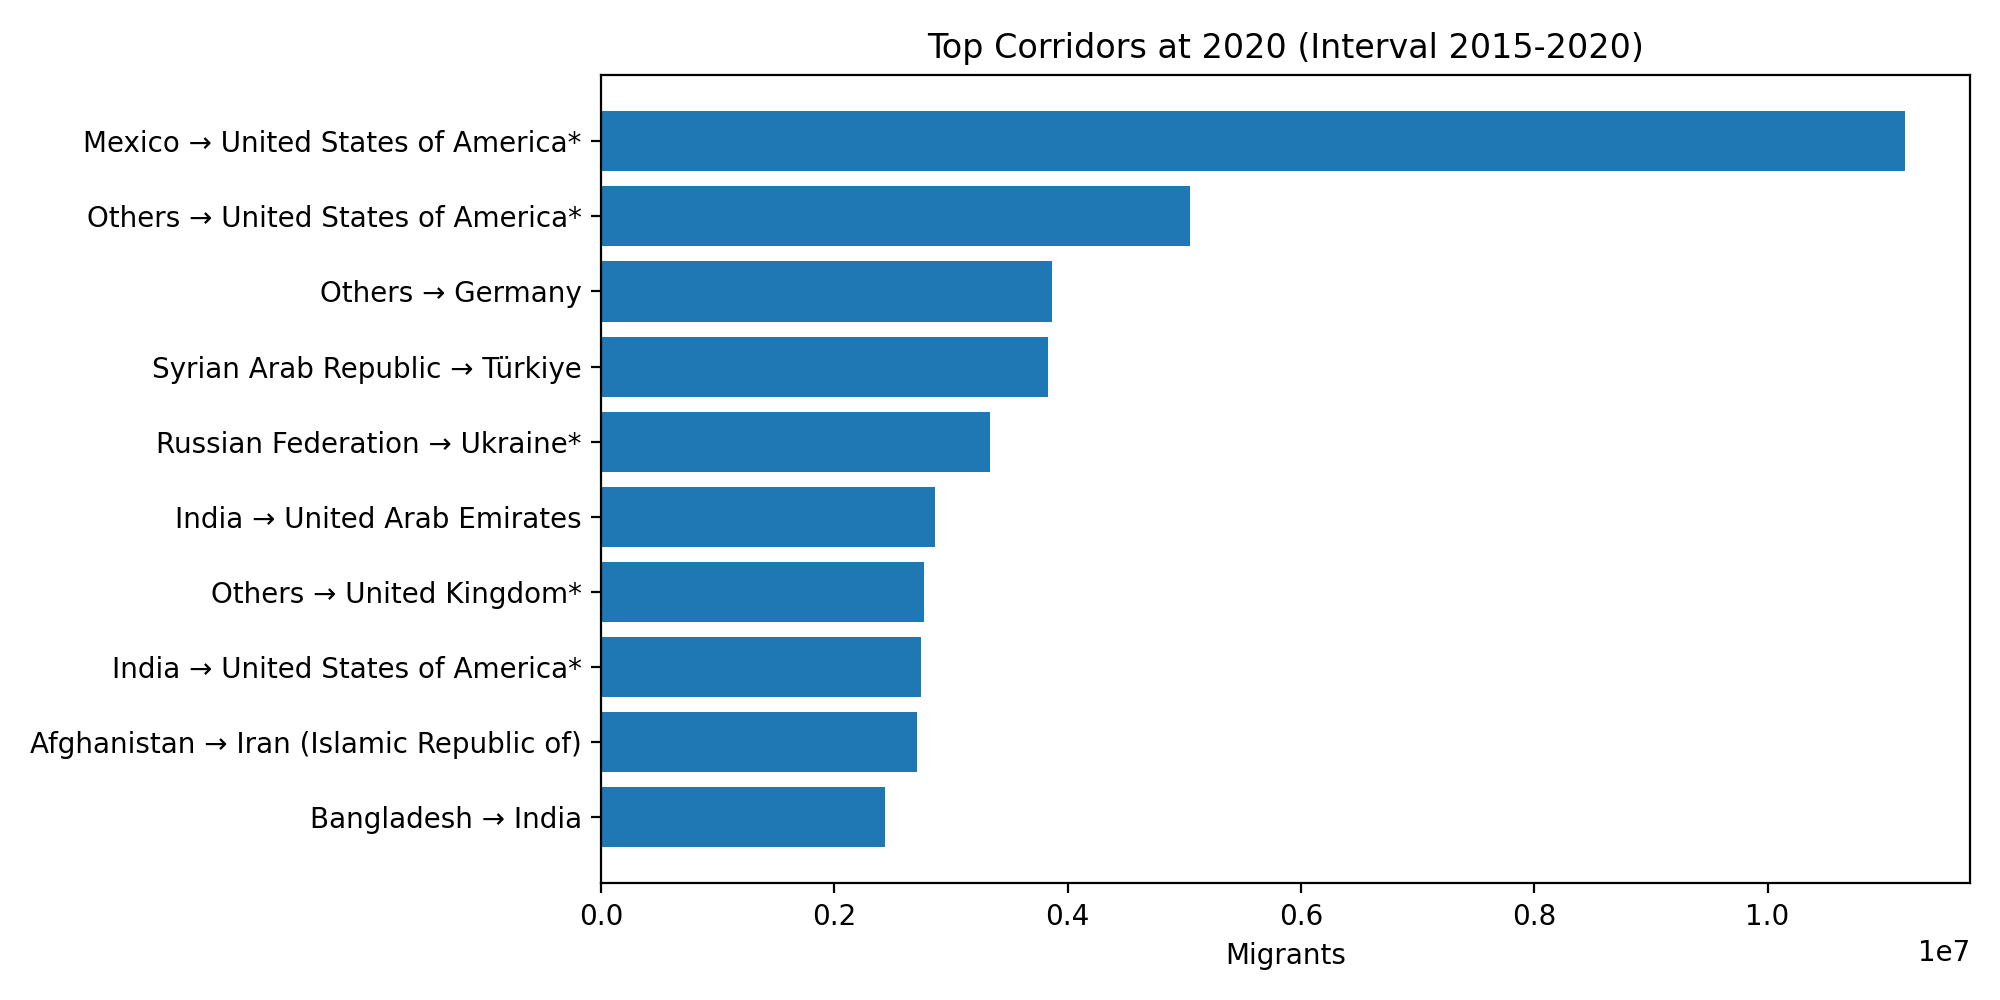
\includegraphics[width=0.95\textwidth]{interval_top_corridors_2015_2020.png}
  \caption{Top migration corridors, 2015--2020.}
\end{figure}

\chapter{Centrality Analysis}
Centrality reveals structural influence, distinguishing global hubs from regional bridges. In-degree captures diversity of inflows, out-degree reflects dispersion of outflows, betweenness highlights brokerage, and PageRank measures global influence. To emphasize both influence and magnitude, we compute a Migration Influence Score (MIS) that weights PageRank by total flow volume.

\[
	ext{MIS(country)} = \text{PageRank(country)} \times \text{Total Flow(country)}
\]

\begin{lstlisting}
import pandas as pd
import networkx as nx

in_deg = nx.in_degree_centrality(G)
out_deg = nx.out_degree_centrality(G)
betw = nx.betweenness_centrality(G, weight="weight", normalized=True)
pr = nx.pagerank(G, weight="weight")

centrality_df = pd.DataFrame({
    "country": list(G.nodes),
    "in_degree": [in_deg[n] for n in G.nodes],
    "out_degree": [out_deg[n] for n in G.nodes],
    "betweenness": [betw[n] for n in G.nodes],
    "pagerank": [pr[n] for n in G.nodes],
})
\end{lstlisting}

  \textbf{Interpretation.} Centrality is not only a structural measure but a proxy for migration behavior. The USA, Germany, and the UK consistently rank high in in-degree and PageRank, reflecting diversified inflow portfolios and sustained institutional pull. Gulf states (UAE, Saudi Arabia, Qatar) appear as concentrated high-inflow hubs driven by contract labor systems and strong corridor specialization, which elevates their PageRank despite smaller populations. High betweenness countries often sit at regional crossroads (e.g., T\"urkiye, Malaysia, South Africa), indicating bridging roles that stabilize corridor connectivity. The concentration of high centrality in a small set of nodes reveals a hub-dominated system rather than a uniformly connected network.

\section*{Insight Summary}
\begin{itemize}
  \item \textbf{Observation:} PageRank and in-degree concentrate in a few destinations. \textbf{Pattern:} a tight core dominates inflows. \textbf{Meaning:} global migration is anchored by a small set of institutional magnets.
  \item \textbf{Observation:} betweenness peaks at regional crossroads. \textbf{Pattern:} connectivity depends on bridge nodes. \textbf{Meaning:} corridor resilience hinges on a few strategic intermediaries.
\end{itemize}

\begin{figure}[H]
  \centering
  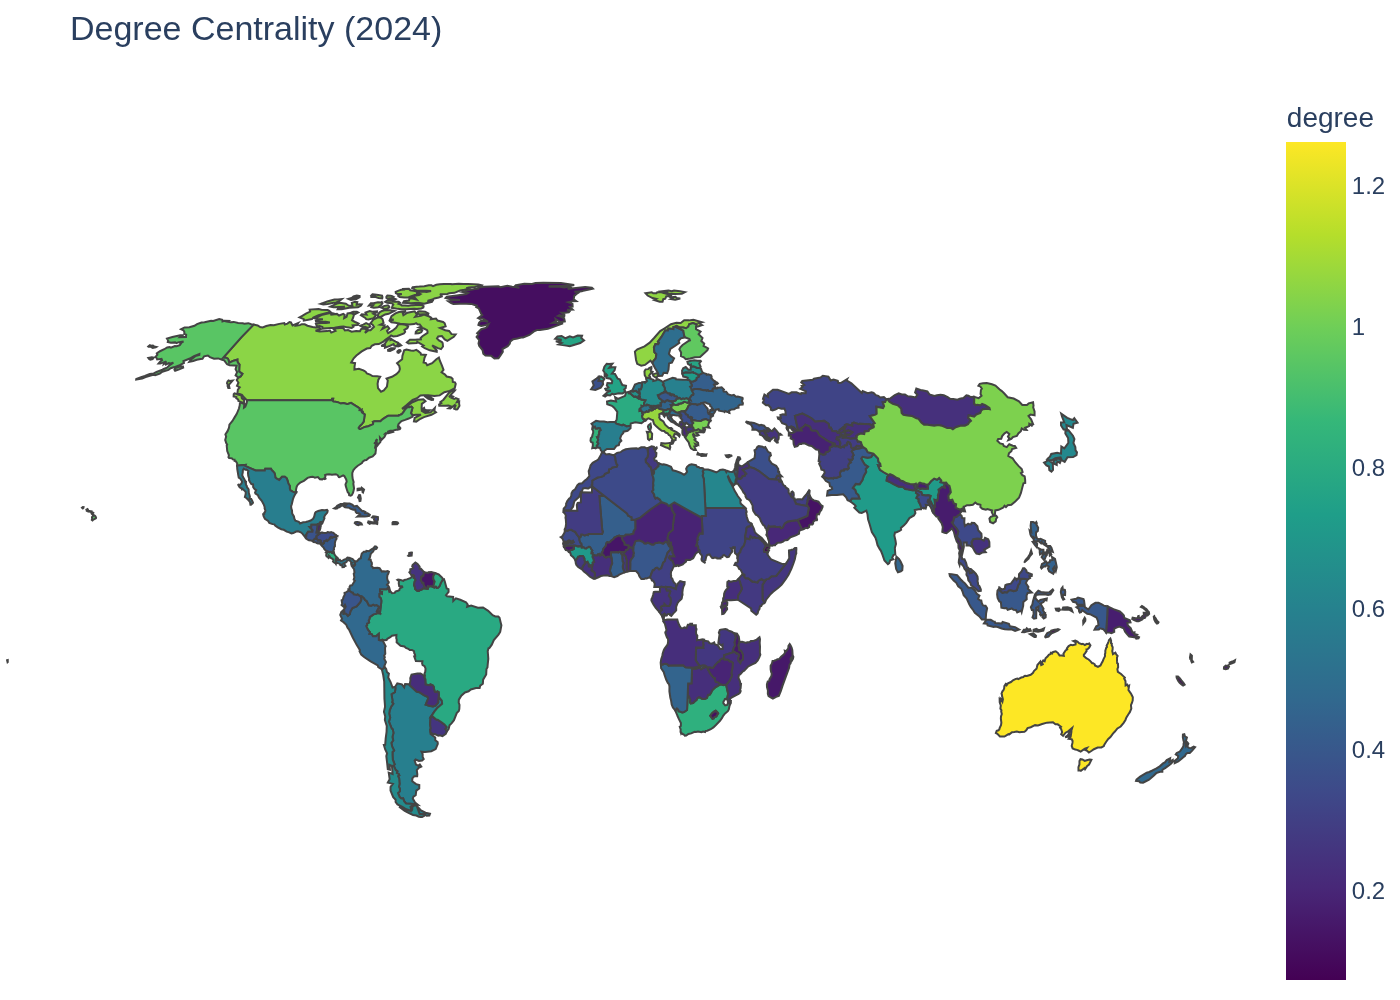
\includegraphics[width=0.9\textwidth]{map_degree.png}
  \caption{Degree centrality map (2024).}
\end{figure}

\begin{figure}[H]
  \centering
  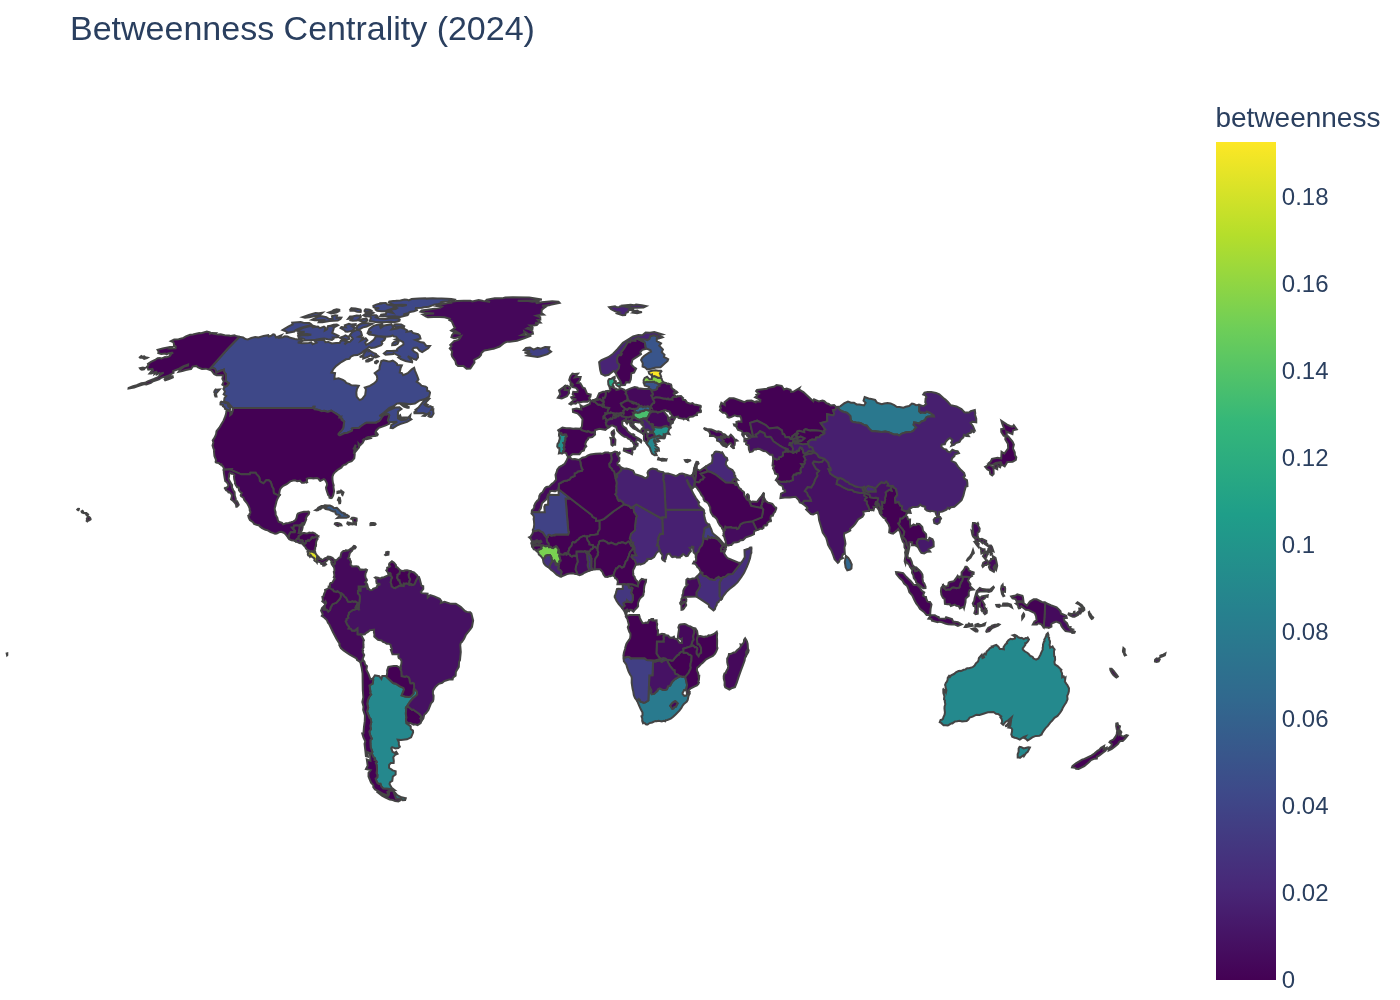
\includegraphics[width=0.9\textwidth]{map_betweenness.png}
  \caption{Betweenness centrality map (2024).}
\end{figure}

\begin{figure}[H]
  \centering
  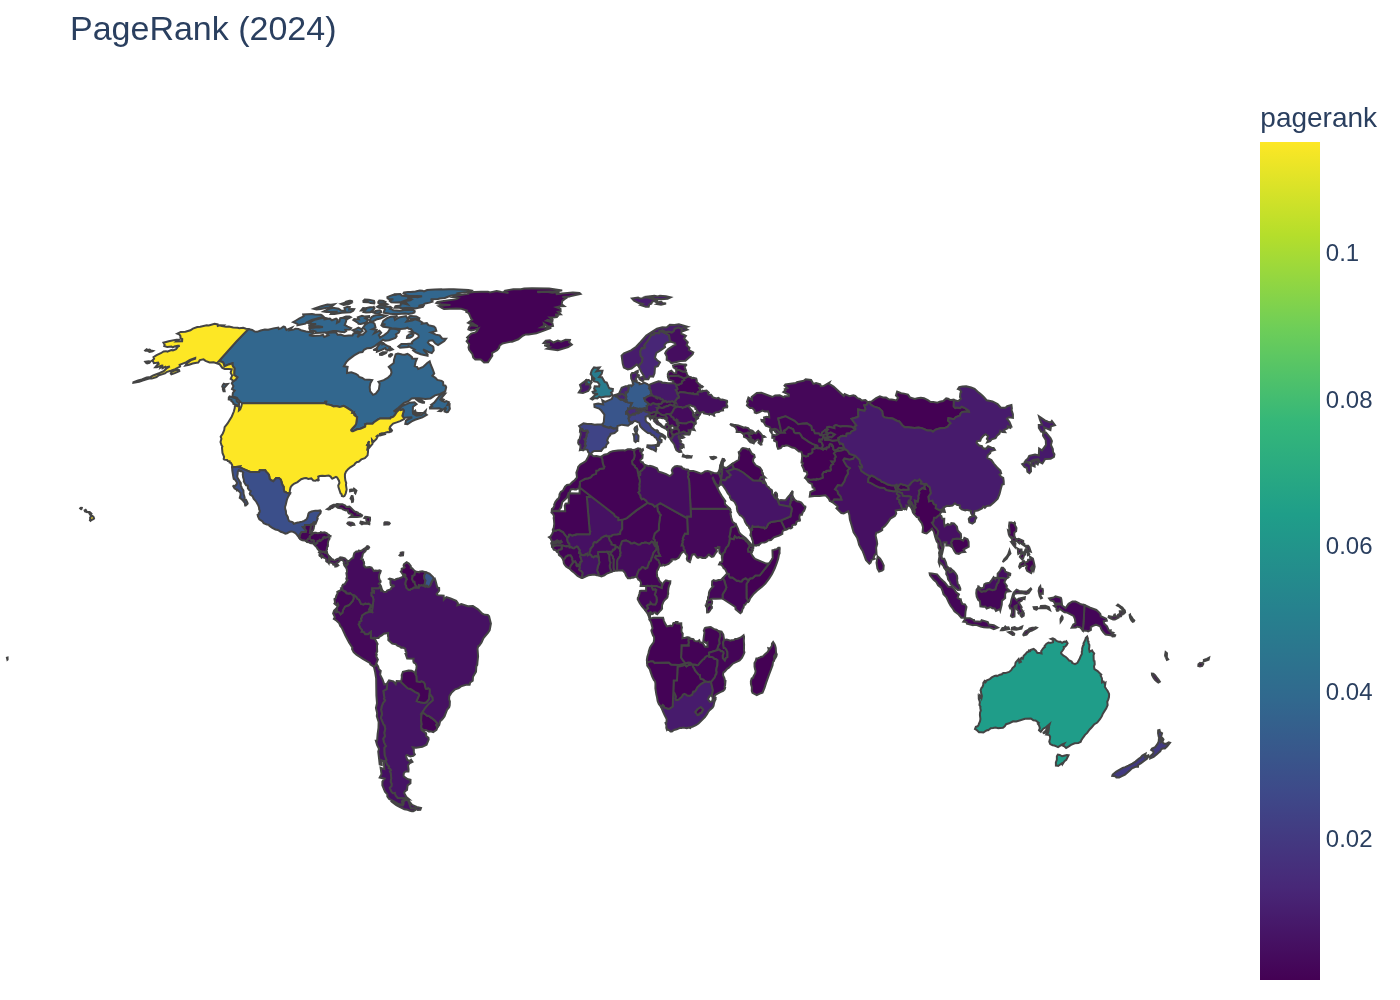
\includegraphics[width=0.9\textwidth]{map_pagerank.png}
  \caption{PageRank centrality map (2024).}
\end{figure}

\chapter{Community Detection}
Community detection uncovers migration blocs with dense internal flows. The goal is to reveal regional systems and corridor clustering that are not obvious from individual edges.

\section{Methods}
	\textbf{Louvain} greedily optimizes modularity by aggregating nodes into communities and compressing the network iteratively. \textbf{Leiden} improves on Louvain by enforcing well-connected communities and avoiding disconnected partitions. \textbf{Girvan--Newman} removes edges with the highest betweenness to expose hierarchical splits, making it a useful baseline for comparison.

\begin{lstlisting}
import community as community_louvain
from networkx.algorithms.community import girvan_newman
from networkx.algorithms.community.quality import modularity

H = G.to_undirected()

louvain_part = community_louvain.best_partition(H, weight="weight")
communities = next(girvan_newman(H))
GN_mod = modularity(H, communities, weight="weight")
\end{lstlisting}

\section{Modularity Comparison}
Modularity is used to compare partitions across methods. In practice, Louvain and Leiden tend to yield clearer, higher-modularity partitions than Girvan--Newman for dense weighted migration graphs, while Girvan--Newman is valuable for interpretability of early splits. Consistent modularity across snapshots indicates stable regional systems.

\section{Interpretation}
Communities align with geography and labor-market linkages: a European cluster centered on Germany and the UK, a Gulf migration system driven by South and Southeast Asian origins, and Latin American corridors anchored to the USA and regional hubs. South--South migration clusters remain visible, reflecting regional mobility and proximity-driven flows. Community stability over time suggests that while corridors evolve, regional blocs persist due to shared language, policy regimes, and historical ties.

\section*{Insight Summary}
\begin{itemize}
  \item \textbf{Observation:} communities map tightly to regions. \textbf{Pattern:} high intra-bloc density. \textbf{Meaning:} migration is regionally segmented by language, policy, and distance.
  \item \textbf{Observation:} Gulf cluster links South and Southeast Asia to a small set of destinations. \textbf{Pattern:} corridor specialization. \textbf{Meaning:} labor systems create predictable, repeatable mobility channels.
\end{itemize}

\begin{figure}[H]
  \centering
  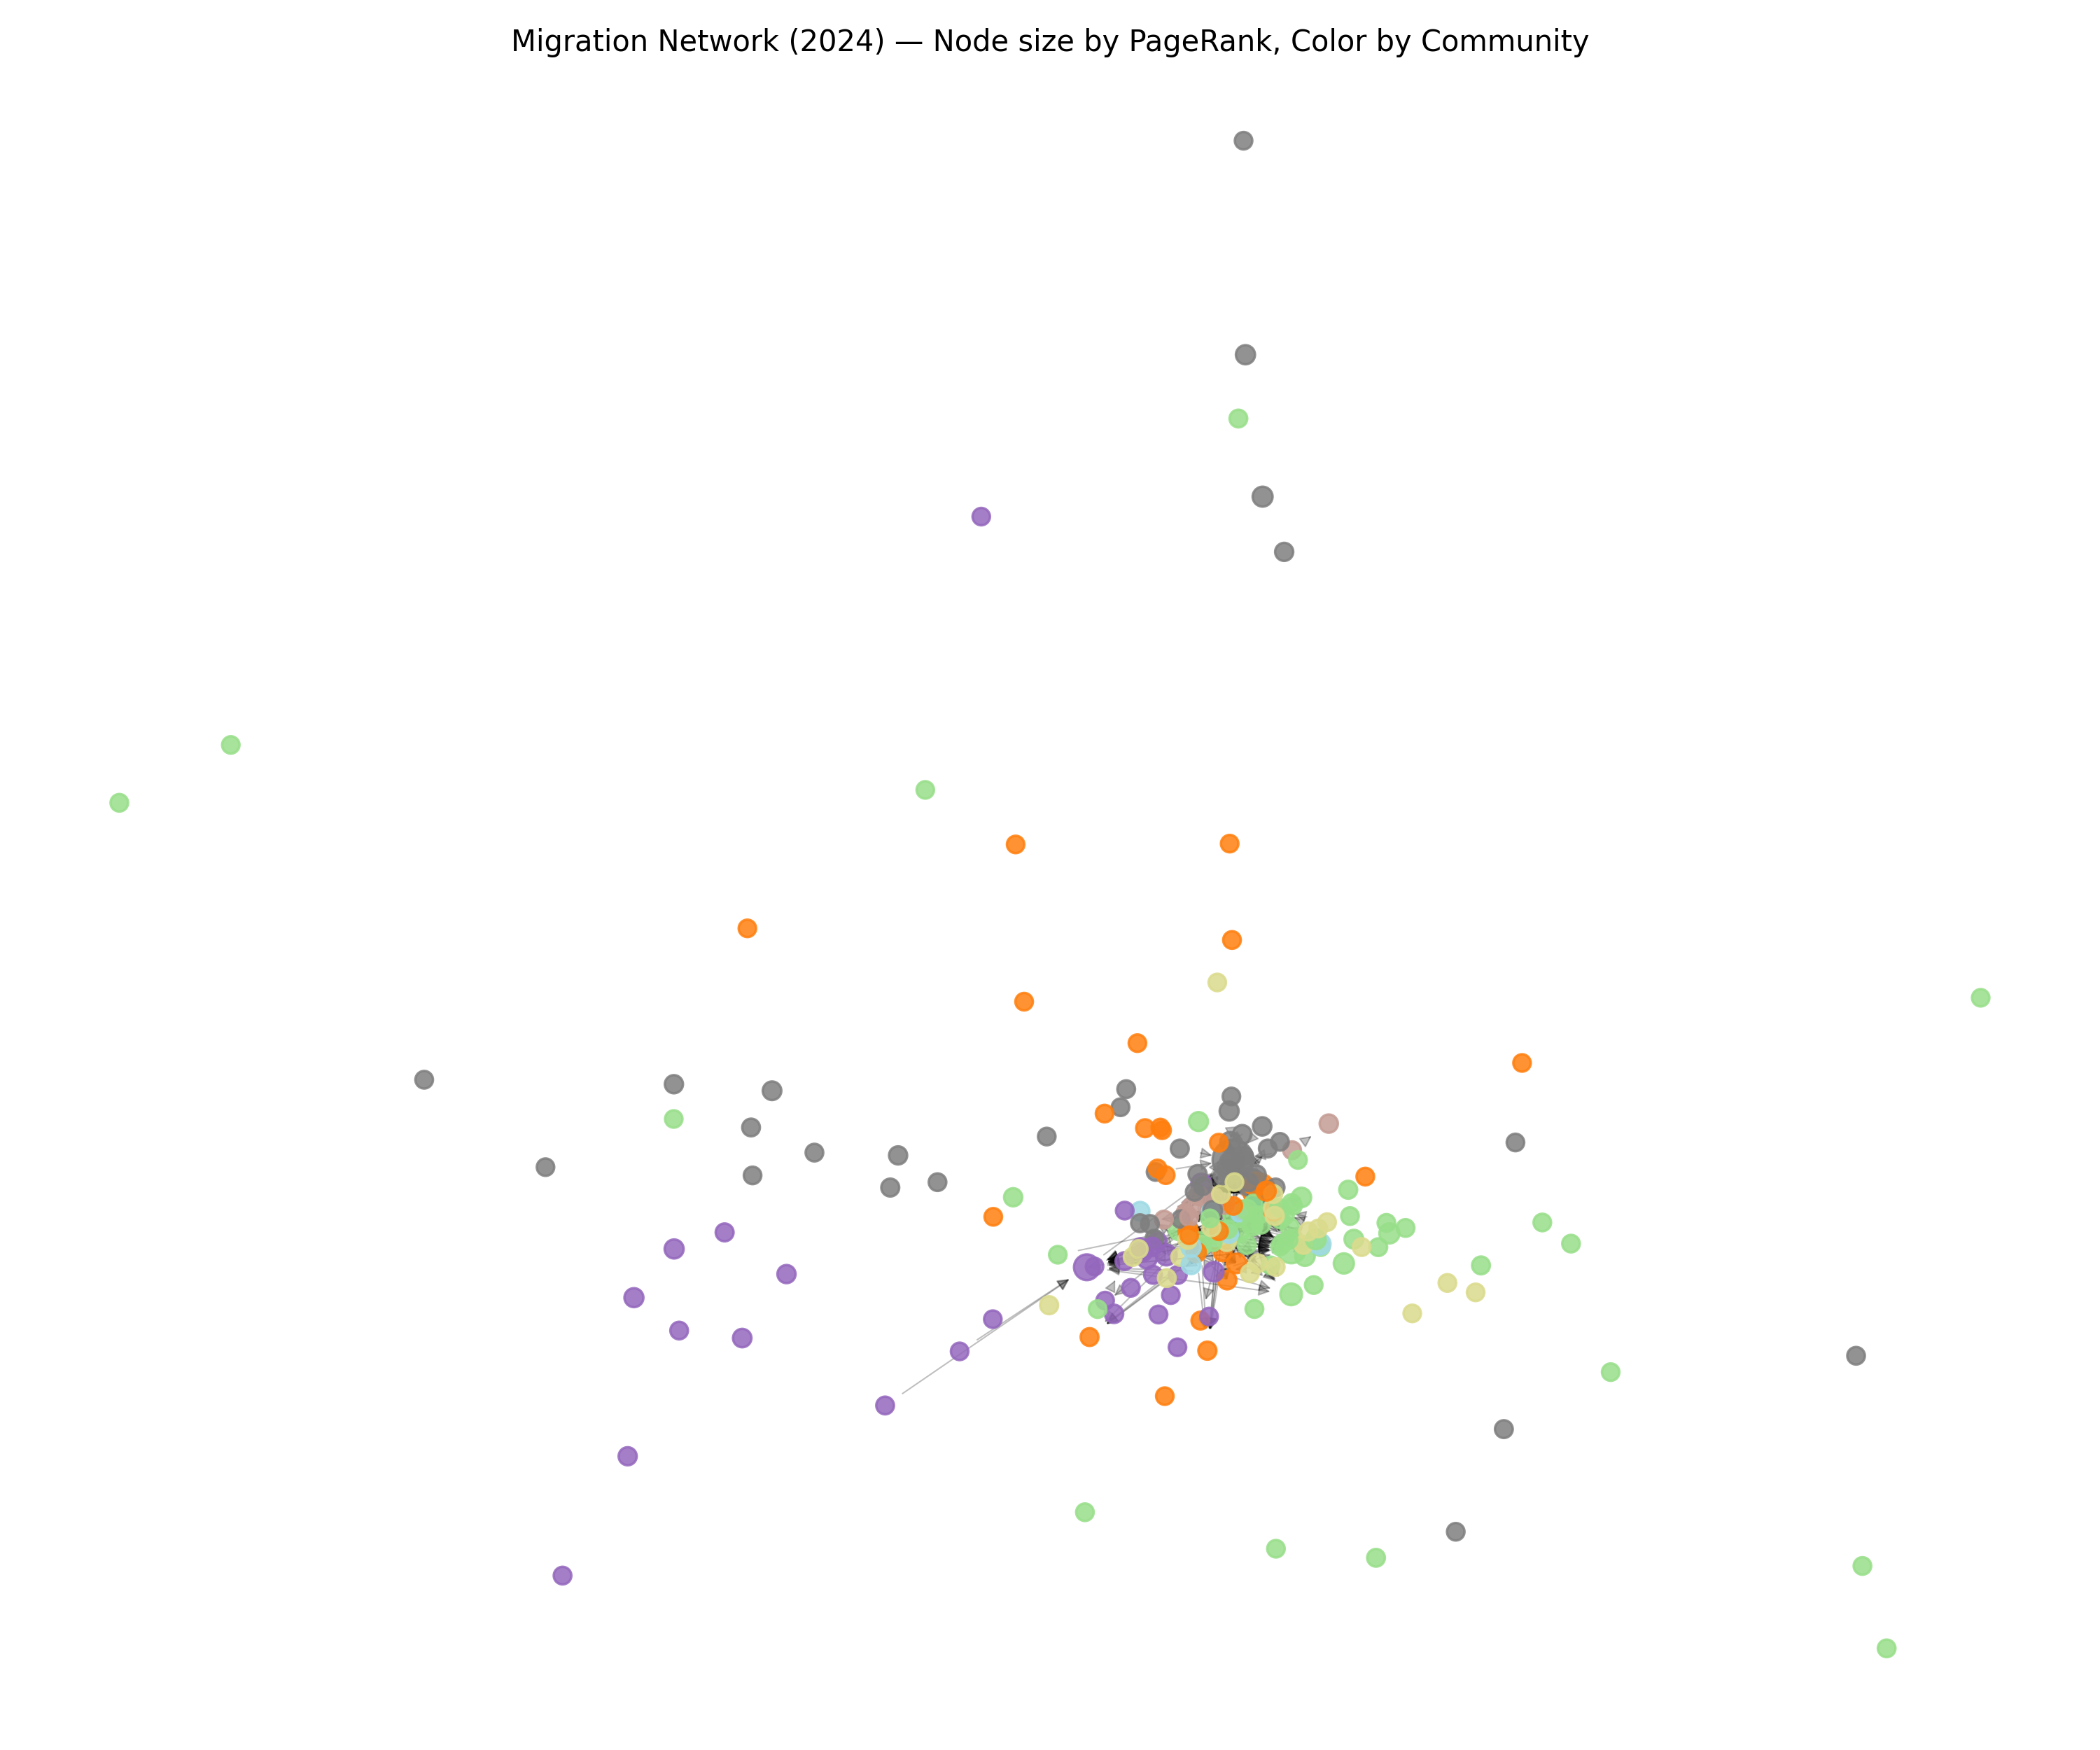
\includegraphics[width=0.9\textwidth]{network_pagerank_community.png}
  \caption{Network visualization with PageRank scaling and community coloring.}
\end{figure}

\chapter{Regression Analysis}
Regression quantifies socio-economic drivers of migration intensity. A log-linear specification stabilizes variance and supports elasticity-style interpretation for scale variables. The dependent variable is $\log(1 + \text{migrants})$, and predictors include GDP, population, unemployment, education, conflict, climate risk, and visa openness. Missing values are imputed with medians and multicollinearity is checked using VIF.

\begin{lstlisting}
import numpy as np
import statsmodels.api as sm

Y = np.log1p(df["migrants"])
features = ["GDP", "population", "unemployment", "education", "conflict", "climate", "visa_openness"]
X = df[features].fillna(df[features].median())
X["GDP"] = np.log1p(X["GDP"])
X["population"] = np.log1p(X["population"])
X = sm.add_constant(X)

model = sm.OLS(Y, X).fit()
print(model.summary())
\end{lstlisting}

  \textbf{Interpretation.} GDP and population typically exhibit positive elasticities, reflecting economic pull and scale effects at destinations. Conflict and climate risks increase outflows from vulnerable origins, while visa openness amplifies corridor intensity by lowering administrative friction. These effects align with push--pull dynamics and highlight how policy accessibility can mediate structural pressures.

\section*{Insight Summary}
\begin{itemize}
  \item \textbf{Observation:} GDP and population are consistently positive. \textbf{Pattern:} scale-driven attraction. \textbf{Meaning:} economic mass, not just policy, anchors global hubs.
  \item \textbf{Observation:} conflict and climate are positive for outflows. \textbf{Pattern:} displacement shocks propagate into corridors. \textbf{Meaning:} crises are structural drivers, not temporary noise.
  \item \textbf{Observation:} visa openness strengthens flows. \textbf{Pattern:} friction reduction amplifies existing routes. \textbf{Meaning:} policy levers can reshape corridor intensity.
\end{itemize}

\chapter{Visualization and Dashboard Design}
The visual layer is an analytical interface that links metrics to migration behavior. Dashboard views triangulate centrality, corridor persistence, and temporal shifts, enabling rapid comparison of hubs, routes, and regional systems.

\section*{Insights from Visual Outputs}
\begin{itemize}
  \item \textbf{Executive overview:} reveals a concentrated destination core, confirming that influence is structurally centralized rather than evenly distributed.
  \item \textbf{Corridor ranking:} separates persistent labor corridors from conflict-driven spikes, indicating which routes are structurally embedded versus episodic.
  \item \textbf{Temporal panels:} show stepwise growth, implying that policy and geopolitical shocks are primary drivers of reconfiguration.
  \item \textbf{Community views:} highlight geographically coherent blocs and limited cross-bloc links, reinforcing regional migration systems.
  \item \textbf{Centrality maps:} align high PageRank with diversified inflow portfolios and elevated betweenness with corridor intermediaries.
\end{itemize}

\begin{figure}[H]
  \centering
  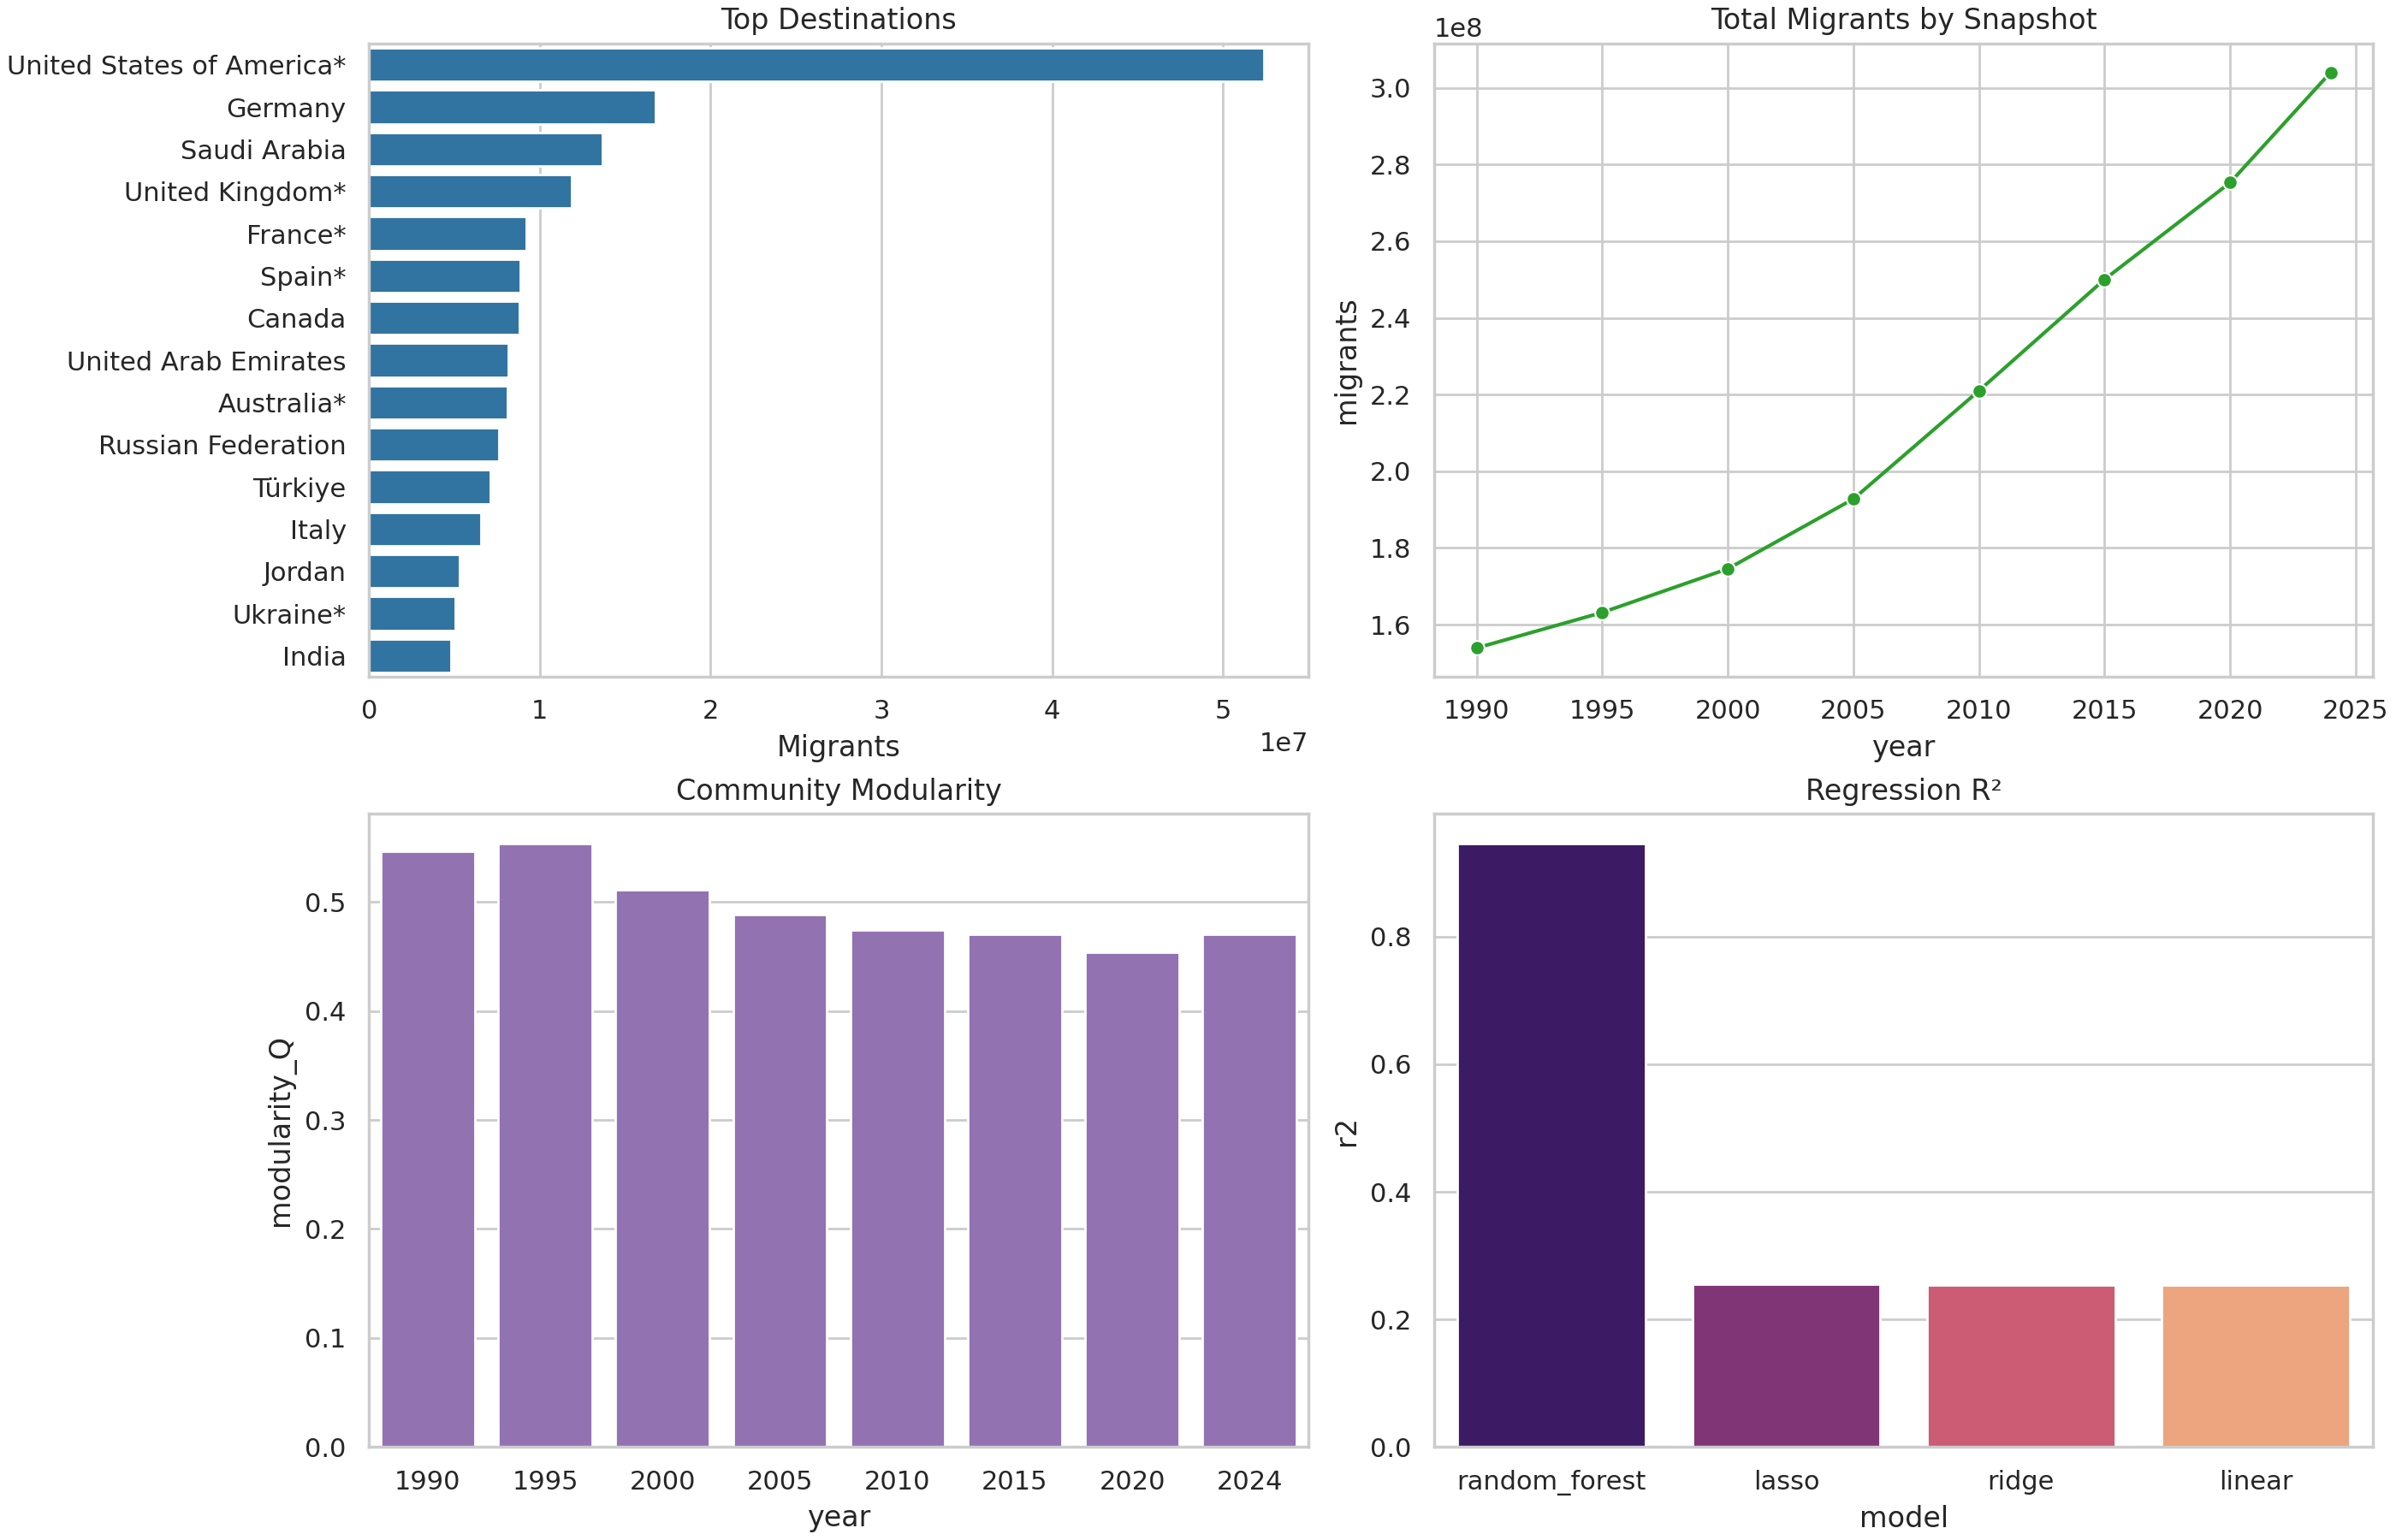
\includegraphics[width=0.95\textwidth]{dashboard_01_overview.png}
  \caption{Power BI Executive Overview dashboard.}
\end{figure}

\begin{figure}[H]
  \centering
  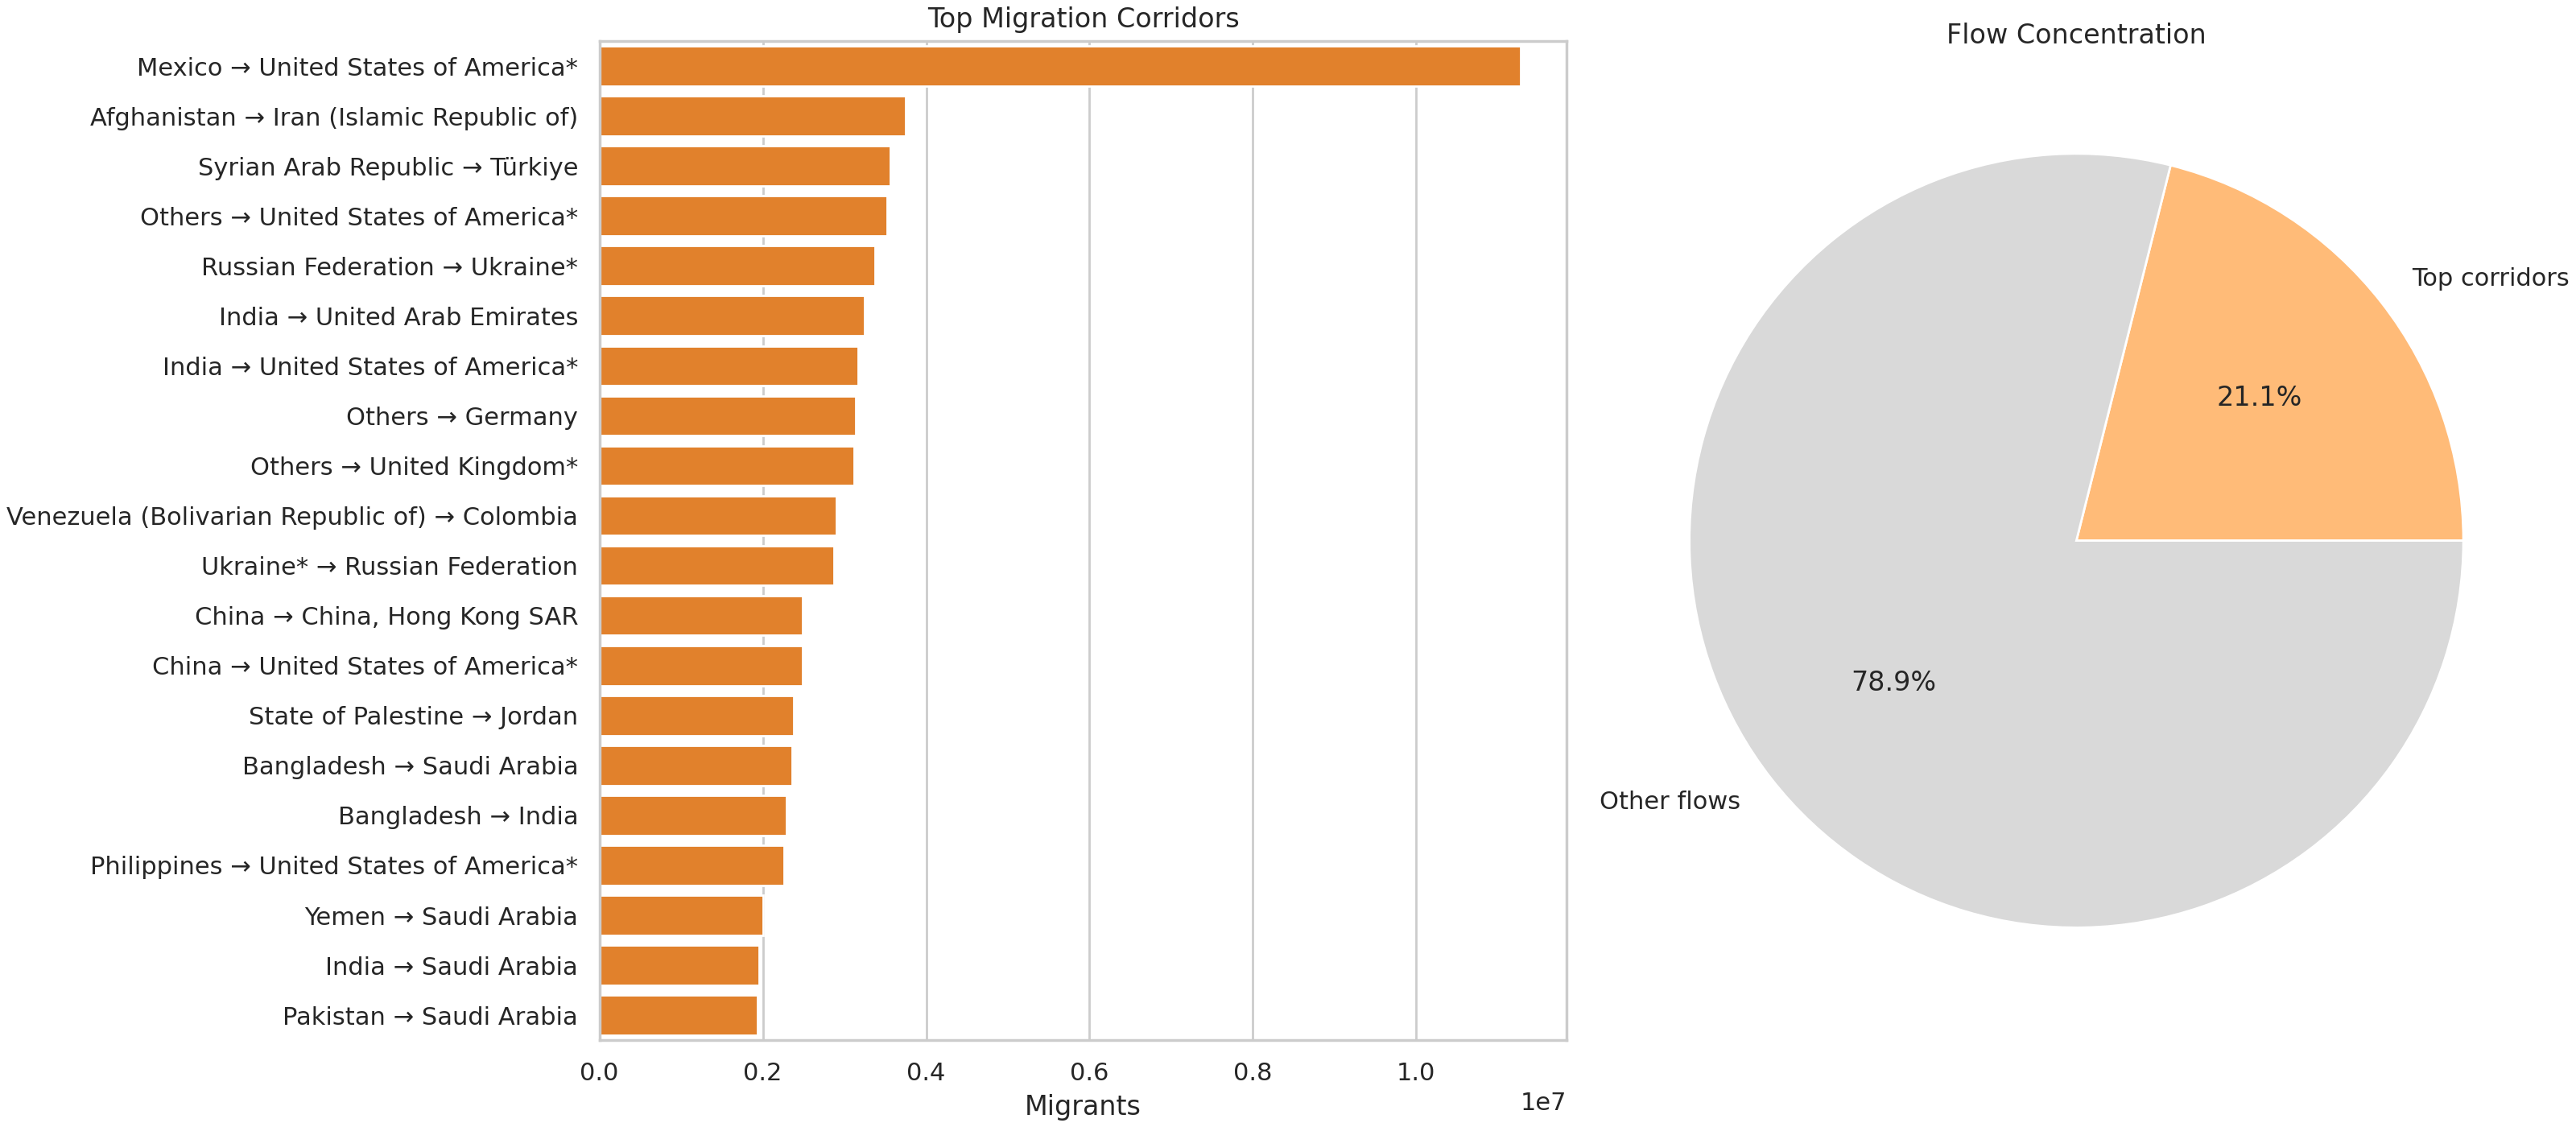
\includegraphics[width=0.95\textwidth]{dashboard_02_corridors.png}
  \caption{Power BI Corridor Analysis dashboard.}
\end{figure}

\chapter{Results and Discussion}
	\textbf{Data $\rightarrow$ Network Measures $\rightarrow$ Patterns $\rightarrow$ Meaning.} The UN DESA bilateral stocks are transformed into temporal networks, and structural measures (centrality, community structure, and regression coefficients) translate raw counts into interpretable migration mechanisms.

\section{Integrated Findings}
Temporal corridor analysis reveals persistent labor and diaspora pathways (e.g., Mexico $\rightarrow$ USA, India $\rightarrow$ UAE), while shock-driven corridors (e.g., Syria $\rightarrow$ T\"urkiye) surge and remain prominent due to proximity and policy responses. Centrality shows that a small set of destinations consistently dominate inflows and influence, indicating concentrated global pull rather than evenly distributed connectivity. Community detection aligns with geography and historical ties, confirming that migration systems are organized into regional blocs with limited cross-bloc bridging. Regression results explain these structural patterns: GDP and population scale the gravitational pull of destinations, conflict and climate pressure intensify outflows, and visa openness amplifies existing corridors.

\section{Key Findings (Analytical Interpretation)}
\begin{itemize}
  \item \textbf{Corridor persistence reflects institutionalized mobility:} stable top corridors indicate long-run labor-market complementarities and policy routinization rather than transient shocks.
  \item \textbf{Hubs are not only large but structurally influential:} high PageRank countries (USA, Germany, UK, UAE, Saudi Arabia) combine diversified inflows with ties to other central nodes, reinforcing their global role.
  \item \textbf{Bridging countries stabilize regional connectivity:} elevated betweenness in regional crossroads suggests that corridor resilience depends on a few intermediary nodes.
  \item \textbf{Community structure is geographically coherent:} Europe, the Gulf, and Latin America emerge as distinct migration systems, with measurable stability across snapshots.
  \item \textbf{Drivers align with push--pull mechanisms:} economic scale and openness pull migrants into hubs, while conflict and climate stress push migrants along emergent corridors.
\end{itemize}

\section*{What this section solves}
\begin{itemize}
  \item \textbf{Problem:} many metrics but no unified story. \textbf{Solved by:} linking temporal corridors, centrality, communities, and regression into one causal narrative.
  \item \textbf{Problem:} patterns without policy meaning. \textbf{Solved by:} mapping results to hubs, bridges, and shock-driven corridors.
\end{itemize}

\section*{High-Impact Analytical Insights}
\begin{itemize}
  \item \textbf{Metric/analysis:} PageRank and in-degree. \textbf{Pattern:} a small destination core dominates inflows. \textbf{Meaning:} global migration is structurally centralized around institutional magnets.
  \item \textbf{Metric/analysis:} Betweenness. \textbf{Pattern:} regional crossroads carry disproportionate brokerage. \textbf{Meaning:} corridor resilience depends on a few intermediaries that connect blocs.
  \item \textbf{Metric/analysis:} Temporal corridor rankings. \textbf{Pattern:} persistent routes remain dominant across intervals. \textbf{Meaning:} long-run labor complementarities and diaspora networks lock in corridors.
  \item \textbf{Metric/analysis:} Interval deltas. \textbf{Pattern:} sharp, stepwise changes rather than smooth growth. \textbf{Meaning:} policy and geopolitical shocks, not gradual drift, reconfigure systems.
  \item \textbf{Metric/analysis:} Community detection. \textbf{Pattern:} coherent regional blocs with limited cross-links. \textbf{Meaning:} migration is organized into regional systems shaped by language, policy, and distance.
  \item \textbf{Metric/analysis:} Regression drivers. \textbf{Pattern:} GDP/population pull and conflict/climate push. \textbf{Meaning:} economic mass anchors hubs while crises redirect flows into emergent corridors.
  \item \textbf{Metric/analysis:} MIS (PageRank $\times$ flow). \textbf{Pattern:} a compact set of high-influence, high-volume nodes. \textbf{Meaning:} policy impact is maximized by focusing on structurally pivotal hubs.
\end{itemize}

\chapter{Applications}
\begin{itemize}
  \item \textbf{Policy design:} prioritize bilateral agreements for dominant corridors.
  \item \textbf{Labor planning:} use hub rankings to allocate resources for integration.
  \item \textbf{Humanitarian response:} monitor emerging corridors for early warning.
\end{itemize}

\chapter{Limitations}
\begin{itemize}
  \item Stock data do not directly measure annual flows, which limits interpretation of short-term shocks and obscures immediate responses to crises.
  \item Recent years (2021--2025) rely on extrapolation and partial updates, introducing uncertainty in late-interval comparisons and dampening detection of emerging corridors.
  \item Informal and undocumented migration are not captured in official bilateral stocks, which underestimates mobility in conflict and low-governance regions.
  \item Missing socio-economic indicators reduce coverage in regression and may bias estimates toward data-rich countries, limiting generalizability across the Global South.
  \item Community detection outcomes depend on resolution parameters and method choice, which can shift boundary assignments and affect cross-snapshot comparability.
\end{itemize}

\chapter{Future Work}
\begin{itemize}
  \item Develop predictive models for corridor evolution using temporal features, conflict indices, and policy variables to address the limits of static snapshots.
  \item Apply dynamic community detection to capture continuous reconfiguration across years and reduce sensitivity to method choice.
  \item Simulate policy interventions (e.g., visa regimes, labor agreements) to test corridor sensitivity and translate findings into decision support.
  \item Integrate flow data and remittance networks to connect mobility with economic feedback loops and better capture short-term shocks.
\end{itemize}

\chapter{Conclusion}
This study demonstrates that global migration is a structured system with a clear core--periphery organization, identifiable hubs, and durable regional blocs. The central contribution is the temporal corridor analysis, which converts bilateral stocks into interval-based dynamics and reveals persistence alongside shock-driven reconfiguration. Centrality and MIS analyses highlight a small set of high-influence, high-volume destinations; community detection shows regionally coherent systems; and regression quantifies how economic scale, conflict, and policy openness jointly shape flows. Together, these findings deliver a cohesive, evidence-based narrative that is directly actionable for migration governance, corridor planning, and early-warning design.

\end{document}
